\section{问题三：共同截面下的第三轮动态资源优化}

\subsection{信息边界与固定赛程}

问题三只处理问题二的 $24$ 场第三轮比赛。比赛编号、双方球队、场馆与开球时段全部锁定，决策仅包括转播优先级 $b_i$、安保等级 $q_i$、交通保障等级 $l_i$ 和票价调整比例 $\delta_i$。前两轮 $48$ 场反馈先汇总成唯一快照，再一次性模拟全部第三轮；任一第三轮模拟结果都不更新其他第三轮比赛参数。因此本问不是按日或按场滚动更新，而是附录图\ref{fig:flow-q3}所示的“共同截面--联合模拟--静动态并行求解--同界复评”。

\subsection{球队状态、进球均值与联合晋级模拟}

球队 $t$ 的前两轮场数、积分和红牌数记为 $G_t,P_t,RC_t$，累计预期进球与累计预期失球记为 $xGF_t,xGA_t$。严格采用题定状态式与伤病截断：
\begin{align}
S_t={}&0.45\frac{P_t}{3G_t}+0.35\left[0.5+0.5\tanh\!\left(\frac{(xGF_t-xGA_t)/G_t}{1.25}\right)\right]
+0.20\exp\!\left(-0.55\frac{RC_t}{G_t}\right),\\
h_t={}&\operatorname{clip}\!\left(\operatorname{mean}_{m\in\mathcal M_t^{1:2}}h_m,0,3\right).
\end{align}
对第三轮比赛 $i=(a,b)$，令
\begin{equation}
\Delta_i=0.32(S_a-S_b)-0.055(h_a-h_b),
\end{equation}
并在基础进球均值上更新
\begin{align}
\lambda_{i,a}&=\operatorname{clip}\!\left(\lambda^0_{i,a}e^{\Delta_i-0.04h_a},0.15,4.50\right),\\
\lambda_{i,b}&=\operatorname{clip}\!\left(\lambda^0_{i,b}e^{-\Delta_i-0.04h_b},0.15,4.50\right).
\end{align}

固定 PCG64 种子后，同时生成 $20000\times24$ 个独立泊松比分。每个样本先在 $12$ 个小组内依次按积分、净胜球、总进球排序，再把 $12$ 个第三名统一比较并选取最好 $8$ 队。完全同分块若跨越晋级线，就按该块可用名额质量等比例分配。因此每次模拟的晋级质量恒等于 $12\times2+8=32$，球队概率满足
\begin{equation}
p_t=\frac{1}{20000}\sum_{m=1}^{20000}w_{tm}^{\mathrm{adv}},qquad
\sum_{t=1}^{48}p_t=32.
\end{equation}
比赛晋级重要性为
\begin{equation}
Q_i=\frac{4p_a(1-p_a)+4p_b(1-p_b)}{2}.
\end{equation}
同一批样本还按本场平局、A 队胜、B 队胜三个条件计算条件晋级概率，用于后续默契风险，而没有再生成另一套不一致的随机样本。

基准种子下 $48$ 队概率位于 $[0.0023,1]$，数值和为 $32.000000$；更新进球均值位于 $[0.4752,3.0146]$。五个固定种子下单队概率标准差最大为 $0.00469$，主要概率位移见图\ref{fig:q3-advancement-shift}。

\begin{figure}[htbp]
    \centering
    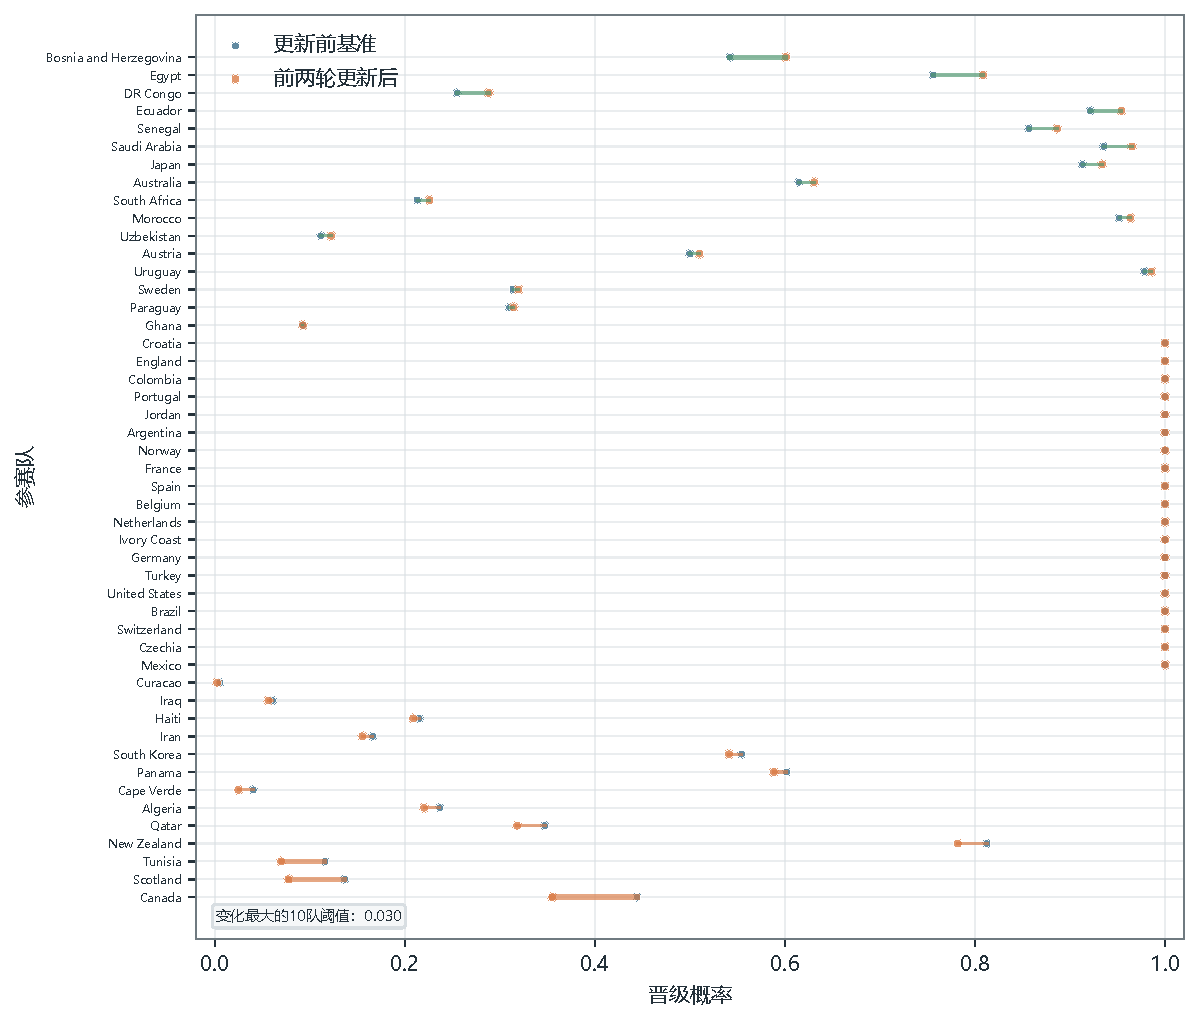
\includegraphics[width=0.82\textwidth,height=0.64\textheight,keepaspectratio]{../figures/fig_q3_advancement_shift.pdf}
    \caption{第三轮开始前的晋级概率更新}
    \label{fig:q3-advancement-shift}
\end{figure}

\subsection{反馈、需求与风险注册表}

对球队 $t$ 的每场前两轮比赛，先把实际/赛前预计现场观众比和转播观众比分别截断到 $[0.60,1.50]$，再取两场均值并截断到 $[0.75,1.25]$，得到 $r_t^N,r_t^V$。比赛层反馈取双方几何平均：
\begin{equation}
f_i^N=\sqrt{r_a^Nr_b^N},\qquad f_i^V=\sqrt{r_a^Vr_b^V}.
\end{equation}
令 $S_i=(S_a+S_b)/2$、$H_i=(h_a+h_b)/6$，以及
\begin{equation}
F_i=\operatorname{clip}\!\left(\frac{0.5f_i^N+0.5f_i^V-0.75}{0.50},0,1\right),
\end{equation}
则吸引力、资源配置前现场需求与转播需求依题定公式更新为
\begin{align}
A_i={}&\operatorname{clip}\!\left(0.50A_i^0+0.25Q_i+0.12F_i+0.08S_i+0.05(1-H_i),0,1\right),\\
\widetilde N_i={}&N_i^{pre}f_i^N(0.88+0.27Q_i)(0.94+0.12S_i)(1-0.10H_i),\\
\widetilde V_i={}&V_i^{pre}f_i^V(0.87+0.30Q_i)(0.90+0.20A_i)(1-0.06H_i).
\end{align}

从资源表读取交通需求倍率 $m_{l_i}^N$、转播需求倍率 $m_{b_i}^V$、安保剩余风险倍率 $m_{q_i}^R$ 和三类成本。附件给出的第三轮价格弹性为 $\varepsilon=-0.75$，票务价值在合法价格域内随 $\delta$ 单调增加，故可先解析消去连续变量：
\begin{equation}
\delta_i^*=\min\left\{\delta_{d(i)}^+,\ 0.88^{1/\varepsilon}-1\right\},
\end{equation}
该值同时满足 $-\delta_{d(i)}^-\le\delta_i^*\le\delta_{d(i)}^+$。最终现场人数、票务价值、转播人数和转播价值为
\begin{align}
N_i(\delta_i^*)&=\min\{K_i,\widetilde N_i m_{l_i}^N(1+\delta_i^*)^{\varepsilon}\},
&TV_i&=P_i^0(1+\delta_i^*)N_i(\delta_i^*),\\
V_i&=\widetilde V_i m_{b_i}^V,
&BV_i&=u_iV_i.
\end{align}
程序逐动作验证 $N_i(\delta_i^*)\ge0.88N_i(0)$，没有把需求底线留到导出后修补。

无激励风险、默契风险、动态安保需求与综合风险分别为
\begin{align}
R_i^{stake}&=0.5(2p_a-1)^2+0.5(2p_b-1)^2,\\
D_i&=\min(p_a^D,p_b^D),\quad
G_i=0.5[p_a^W-p_a^D]_++0.5[p_b^W-p_b^D]_+,\\
R_i^{col}&=\operatorname{clip}\!\left(D_i[1-\operatorname{clip}(G_i,0,1)](1-0.35R_i^{stake}),0,1\right),\\
d_i&=\operatorname{clip}\!\left(0.45d_i^0+0.25O_i+0.15A_i+0.15\frac{R_i^{stake}+R_i^{col}}2,0,1\right),\\
R_i&=0.40R_i^{stake}+0.40R_i^{col}+0.20d_im_{q_i}^R,qquad
O_i=\operatorname{clip}(\widetilde N_i/K_i,0,1).
\end{align}

\subsection{静态基线、动态动作与日级约束}

每场枚举 $b_i\in\{1,2,3\}$、$q_i\in\{L_i^{req},\ldots,L_{v(i)}^{sec}\}$、$l_i\in\{1,2,3\}$，票价取上式解析最优值。资源成本为 $C_i=c_{b_i}+c_{q_i}+c_{l_i}$。在全部更新动作上一次计算 $TV,BV,A,C,R$ 的共同 Min--Max 边界，目标为
\begin{equation}
\max Z_3=\sum_{i\in I_3}\left(0.35TV_i'+0.35BV_i'+0.10A_i'-0.10C_i'-0.10R_i'\right).
\end{equation}
对每个实际出现的参考日 $d$，同时施加
\begin{align}
\sum_{i\in I_d}\mathbf 1(b_i=3)&\le H_d^B,&
\sum_{i\in I_d}\mathbf 1(q_i\ge3)&\le H_d^S,\\
\sum_{i\in I_d}\mathbf 1(l_i=3)&\le H_d^L,&
\sum_{i\in I_d}C_i&\le B_d.
\end{align}

静态方案不是默认档位：它先用赛前需求、赛前吸引力及题定赛前风险，在完全相同的动作集合和日约束下独立优化；前两轮结束后四项决策锁定，只把该动作放入更新环境重评。动态方案则在更新环境中重新优化。两者最终均使用更新动作域的同一组边界计分，故 $Z_3^{static}$ 与 $Z_3^{dynamic}$ 可直接比较；模型中不存在“变更惩罚”或另一套分资源预算。

\begin{table}[H]
\centering
\caption{问题三逐日动态资源使用与容量}
\label{tab:q3-resource-budget}
\small
\resizebox{\textwidth}{!}{%
\begin{tabular}{lrrrrrrrrc}
\toprule
日期 & 高转播 & 转播上限 & 高安保 & 安保上限 & 强化交通 & 交通上限 & 预算使用 & 预算上限 & 状态 \\
\midrule
2026-06-20 & 2 & 4 & 1 & 3 & 2 & 4 & 35.0 & 120 & 通过 \\
2026-06-22 & 1 & 3 & 0 & 3 & 0 & 3 & 13.0 & 100 & 通过 \\
2026-06-23 & 3 & 3 & 3 & 3 & 3 & 3 & 86.0 & 100 & 通过 \\
2026-06-24 & 3 & 3 & 1 & 2 & 3 & 3 & 51.0 & 100 & 通过 \\
2026-06-28 & 4 & 4 & 3 & 3 & 4 & 4 & 77.0 & 120 & 通过 \\
2026-06-29 & 3 & 3 & 2 & 2 & 2 & 3 & 54.0 & 100 & 通过 \\
2026-06-30 & 3 & 3 & 2 & 2 & 3 & 3 & 59.0 & 100 & 通过 \\
\bottomrule
\end{tabular}
}
\end{table}


新问题二赛程使第三轮分布在 $7$ 个参考日。表\ref{tab:q3-resource-budget}逐日给出三级转播、三级及以上安保、三级交通和总预算使用量，所有不等式均通过；安保档位还逐场满足最低需求且不超过固定场馆能力。

\subsection{结果、同界增益与随机稳定性}

\begin{table}[H]
\centering
\caption{问题三静态策略与动态重优化同界比较}
\label{tab:q3-static-dynamic}
\small
\begin{tabular}{lrrrr}
\toprule
指标 & 静态策略重评 & 动态重优化 & 偏好方向改善 & 单位 \\
\midrule
票务价值 TV & 113.715 & 113.385 & -0.330 & 百万美元 \\
转播价值 BV & 168.309 & 168.368 & 0.059 & 百万美元 \\
吸引力 A & 0.512 & 0.512 & 0.000 & 无量纲 \\
资源成本 C & 396.000 & 375.000 & 21.000 & 成本指数 \\
风险 R & 0.465 & 0.469 & -0.004 & 无量纲 \\
综合目标 Z3 & 6.572230 & 6.637484 & 0.065254 & 无量纲 \\
\bottomrule
\end{tabular}
\vspace{2pt}
\noindent\begin{minipage}{0.96\textwidth}\footnotesize 注：正的偏好方向改善表示动态方案更优；成本与风险按越低越优转换。\end{minipage}
\end{table}


静态锁定方案在更新环境中的同界得分为 $6.572230$，动态重优化得分为 $6.637484$，净增量为 $0.065254$；$24$ 场中 $8$ 场改变至少一个资源决策。表\ref{tab:q3-static-dynamic}显示，动态方案票务价值减少 $0.330$ 百万美元、转播价值增加 $0.059$ 百万美元、资源成本指数减少 $21$，风险均值增加约 $0.004$。因此增益来自题定五指标的全局权衡，而不是不存在的改动成本。

\begin{figure}[htbp]
    \centering
    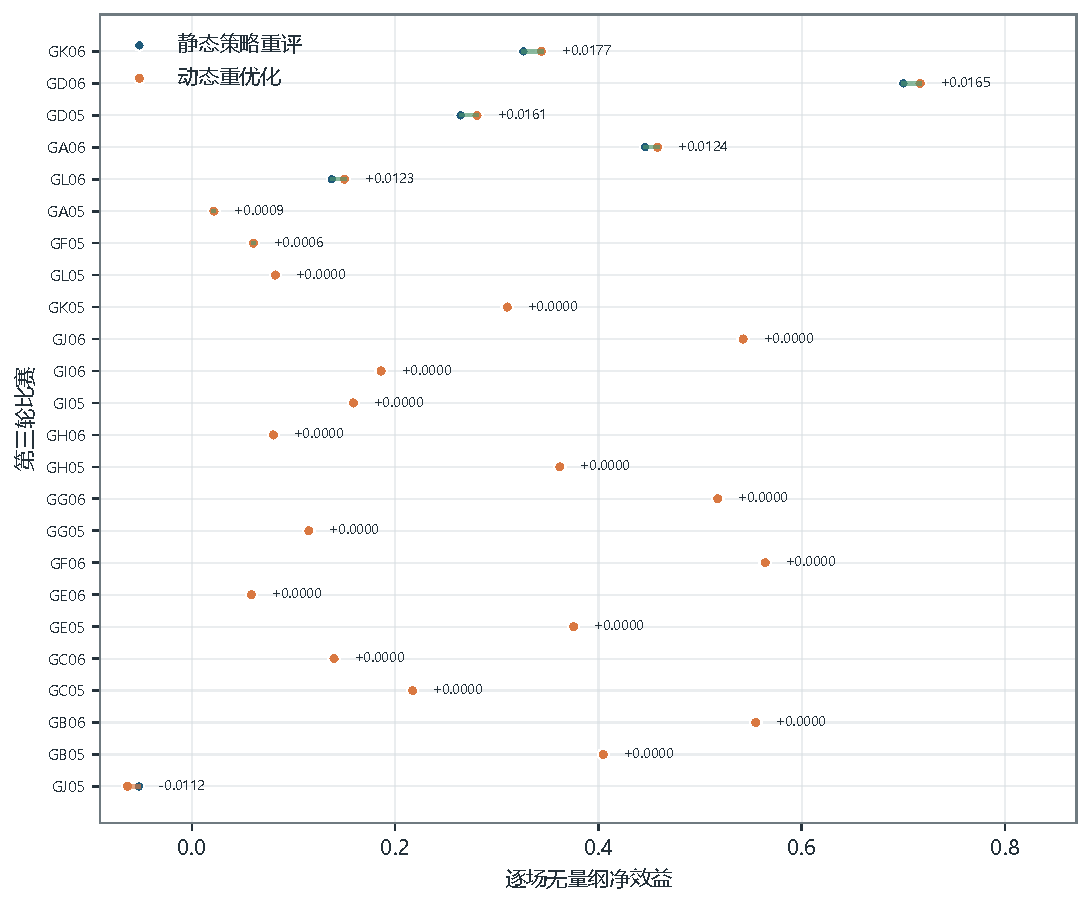
\includegraphics[width=0.84\textwidth,height=0.66\textheight,keepaspectratio]{../figures/fig_q3_dynamic_value_dumbbell.pdf}
    \caption{静态锁定方案与动态重优化的逐场同界净价值}
    \label{fig:q3-dynamic-value-dumbbell}
\end{figure}

五个种子均重新执行 $20000\times24$ 联合模拟、条件概率计算、环境更新和完整动态 CP-SAT。五次动态求解均为 `OPTIMAL`，增益位于 $[0.065123,0.065434]$，相对基准种子的 $24$ 场动态资源决策均无变化。这说明本次配置差异不是由单个随机种子的抽样波动驱动。
